\documentclass[11pt, a4paper]{article}

%MUST DOWNLOAD algorithm.sty
\usepackage{algorithm} 
%\usepackage{algorithmicx}
\usepackage{algpseudocode}
\usepackage{empheq}
\usepackage{euscript}
\usepackage{amsmath}
\usepackage{amsthm}
\usepackage{amssymb}
\usepackage{epsfig}
\usepackage{xspace}
\usepackage{color}
\usepackage{url}

%\usepackage{algpseudocode}

\usepackage{mathtools}
\DeclarePairedDelimiter\ceil{\lceil}{\rceil}
\DeclarePairedDelimiter\floor{\lfloor}{\rfloor}

%%%%%%%  For drawing trees  %%%%%%%%%
\usepackage{tikz}
\usetikzlibrary{calc, shapes, backgrounds}

%%%%%%%%%%%%%%%%%%%%%%%%%%%%%%%%%
\setlength{\textheight}{9in}
\setlength{\topmargin}{-0.600in}
\setlength{\headheight}{0.2in}
\setlength{\headsep}{0.250in}
\setlength{\footskip}{0.5in}
\flushbottom
\setlength{\textwidth}{6.5in}
\setlength{\oddsidemargin}{0in}
\setlength{\evensidemargin}{0in}
\setlength{\columnsep}{2pc}
\setlength{\parindent}{1em}
\setlength\fboxsep{1cm}
%%%%%%%%%%%%%%%%%%%%%%%%%%%%%%%%%


\newcommand{\eps}{\varepsilon}

\renewcommand{\c}[1]{\ensuremath{\EuScript{#1}}}
\renewcommand{\b}[1]{\ensuremath{\mathbb{#1}}}
\newcommand{\s}[1]{\textsf{#1}}
\newcommand*\widefbox[1]{\fbox{\hspace{2em}#1\hspace{2em}}}
\newcommand{\E}{\textbf{\textsf{E}}}
\renewcommand{\Pr}{\textbf{\textsf{Pr}}}
\renewcommand{\labelenumi}{(\alph{enumi}) }


\title{Feedback Exercise 
}
\author{Sameuel Leventhal and Unnikrishnan Rajagopalan}
\date{}

\begin{document}

\maketitle


%%%%%%%%%%%%%%%%%%%%%%%%%%%%%%%%%%%%%%%%%%%%%%%%%%%%
%%%%%%%%%%%%%%%%%%%%%%%%%%%%%%%%%%%%%%%%%%%%%%%%%%%%
%%%%%%%%%%%%%%%%%%%%%%%%%%%%%%%%%%%%%%%%%%%%%%%%%%%%



\iffalse

%
% Image
%
\begin{figure}[H]
\centering{
\includegraphics[width=.8\linewidth]{problem1plot.png}
}
\label{fig:prob1fig}
\end{figure}

%
% Matrix
%
\[ \begin{pmatrix}
  4 & 1 \\
  0 & 4 \\
\end{pmatrix}\]

%
% Algorithm
%
  \begin{algorithm}[H]
\caption{Matrix Inversion by LU decomposition}
\begin{algorithmic}
  \For{$k = 1:n$}
      \For{$i=1:n$}
          \If{$i\neq k$}
              \State $l_{ik} \leftarrow \frac{A_{ik}}{A_{kk}}$ \Comment{(n-1)}
                    \For{$j=k+1 : 2n$}
                        \State $A_{ij} \leftarrow A_{ij} - l_{ik}A_{kj}$ \Comment{2(n-1)(2n-k)}
                    \EndFor
                    \EndIf
                    \For{$j=2n:k$}
                    \State $A_{kj} \leftarrow \frac{A_{kj}}{A_{kk}}$ \Comment{2n-k+1}
                    \EndFor
      \EndFor
  \EndFor
\end{algorithmic}
\end{algorithm}

%
% Another matrix
%
  \[
  \begin{smallmatrix}
    1 & 1 & 1 & \cdots & 1 & 2 & 3 & 4 & \cdots & n & 2 & 3 & \cdots &n\\
    1 & 2 & 3 & \cdots & n & 1 & 1 & 1 & \cdots & 1 & 2 & 3 & \cdots & n\\
    c_{1,1} & c_{1,2} & c_{1,3} & \cdots & c_{1,n} & c_{2,1} & c_{3,1} & c_{4,1} & \cdots & c_{n,1} & c_{2,2} & c_33 &\cdots &c_nn\\
  \end{smallmatrix}
\]

%
% bounding box
%
\noindent\fbox{
  \parbox{.8\textwidth}{

  }
}



\fi

%     End of tex formatting samples. Begin Document   %%%%
%%%%%%%%%%%%%%%%%%%%%%%%%%%%%%%%%%%%%%%%%%%%%%%%%%%%%%%%%%%%%%%%%%%%%%%%%
%%%%%%%%%%%%%%%%%%%%%%%%%%%%%%%%%%%%%%%%%%%%%%%%%%%%%%%%%%%%%%%%%%%%%%%%%
%%%%%%%%%%%%%%%%%%%%%%%%%%%%%%%%%%%%%%%%%%%%%%%%%%%%%%%%%%%%%%%%%%%%%%%%%

\section{ Quality of feedback }

\textbf{Feedback Group:}
\begin{itemize}
\item Shane Brown (u0852900)
\item Sigmund Chow (u0597938)
\item My Huynh (u0729654)
\end{itemize}

We found the feedback given very helpful and informative. Discussing our project illuminated aspects that were convoluted, allowing for new approaches to be either recommended by our reviewers or derived by us. Below are the suggestions or resolved confusions which we believe will provide for a more informative and intuitive visualization:
\begin{enumerate}
\item \textbf{Issue}:The bar charts for each school selected by the user add an extra component of confusion by grouping all top ten attributes for each school since attributes do not share the same units so height comparison is meaningless.
  
  \textbf{Solution}: We have decided to instead of creating a bar chart for each school we can better preserve the main goal of school comparison by making ten bar charts for each of the ``top ten first asked school attribute'' within which is a bar for each of the schools selected by the user. By doing so the user will be able to see how well any of the selected schools performs with respect to the other schools.
\item \textbf{Issue}: There is a level of redundancy by adding a ``Start'' and ``Stop'' button for when a user decides to select a school on the map.

  \textbf{Solution}: It was suggested instead the may select a school on the map which triggers the event of having that schools histogram as well as more detailed attributes to be displayed. After selecting a number of schools the comparisons between schools will all be displayed lower. The User can then remove a school by again selecting the school on the map or selecting a small ``x'' icon by the schools name lower down.

\item \textbf{Issue}: After explaining the attribute comparison in which a range, defined by the max and min value of the selected schools attributes, and each of the selected schools displayed within that range as a circle it was pointed out to us that as more schools are selected it will be difficult to maintain an understanding of how a school falls into a national perspective, i.e. if the range changes for the selected schools picking top 5 worst schools might look similar to the top 5 best schools.

  \textbf{Solution}: We can decided that not only would it be more informative but clearer to add to each attribute comparison in the ``detailed'' section two ranges: the first defined by the domain of the schools selected and the second defined by all schools. In this way as a user selects schools they will be able to see how a school from their selection performs with respect to the other selected schools as well as how the school compares nationally. To better illuminate this on the national scale we will also put a marker along the range indicating national average.
  
  

\end{enumerate}

\section{Other changes decided on}

We no longer will include the option to compare a preset number of schools. Our incentive for this is due to the ambiguity on which schools to select from the total range of each and between all attributes. We are also considering including a protip functionality on which where rather than only displaying the schools name when mousing over it's representative circle on the map it also displays in plain text the exact values of the top ten most asked questions about a school such as ranking, tuition, average acceptance rate, and so on. A sketch is given below on the direction we intend to take this project.

\begin{figure}[h]
\centering{
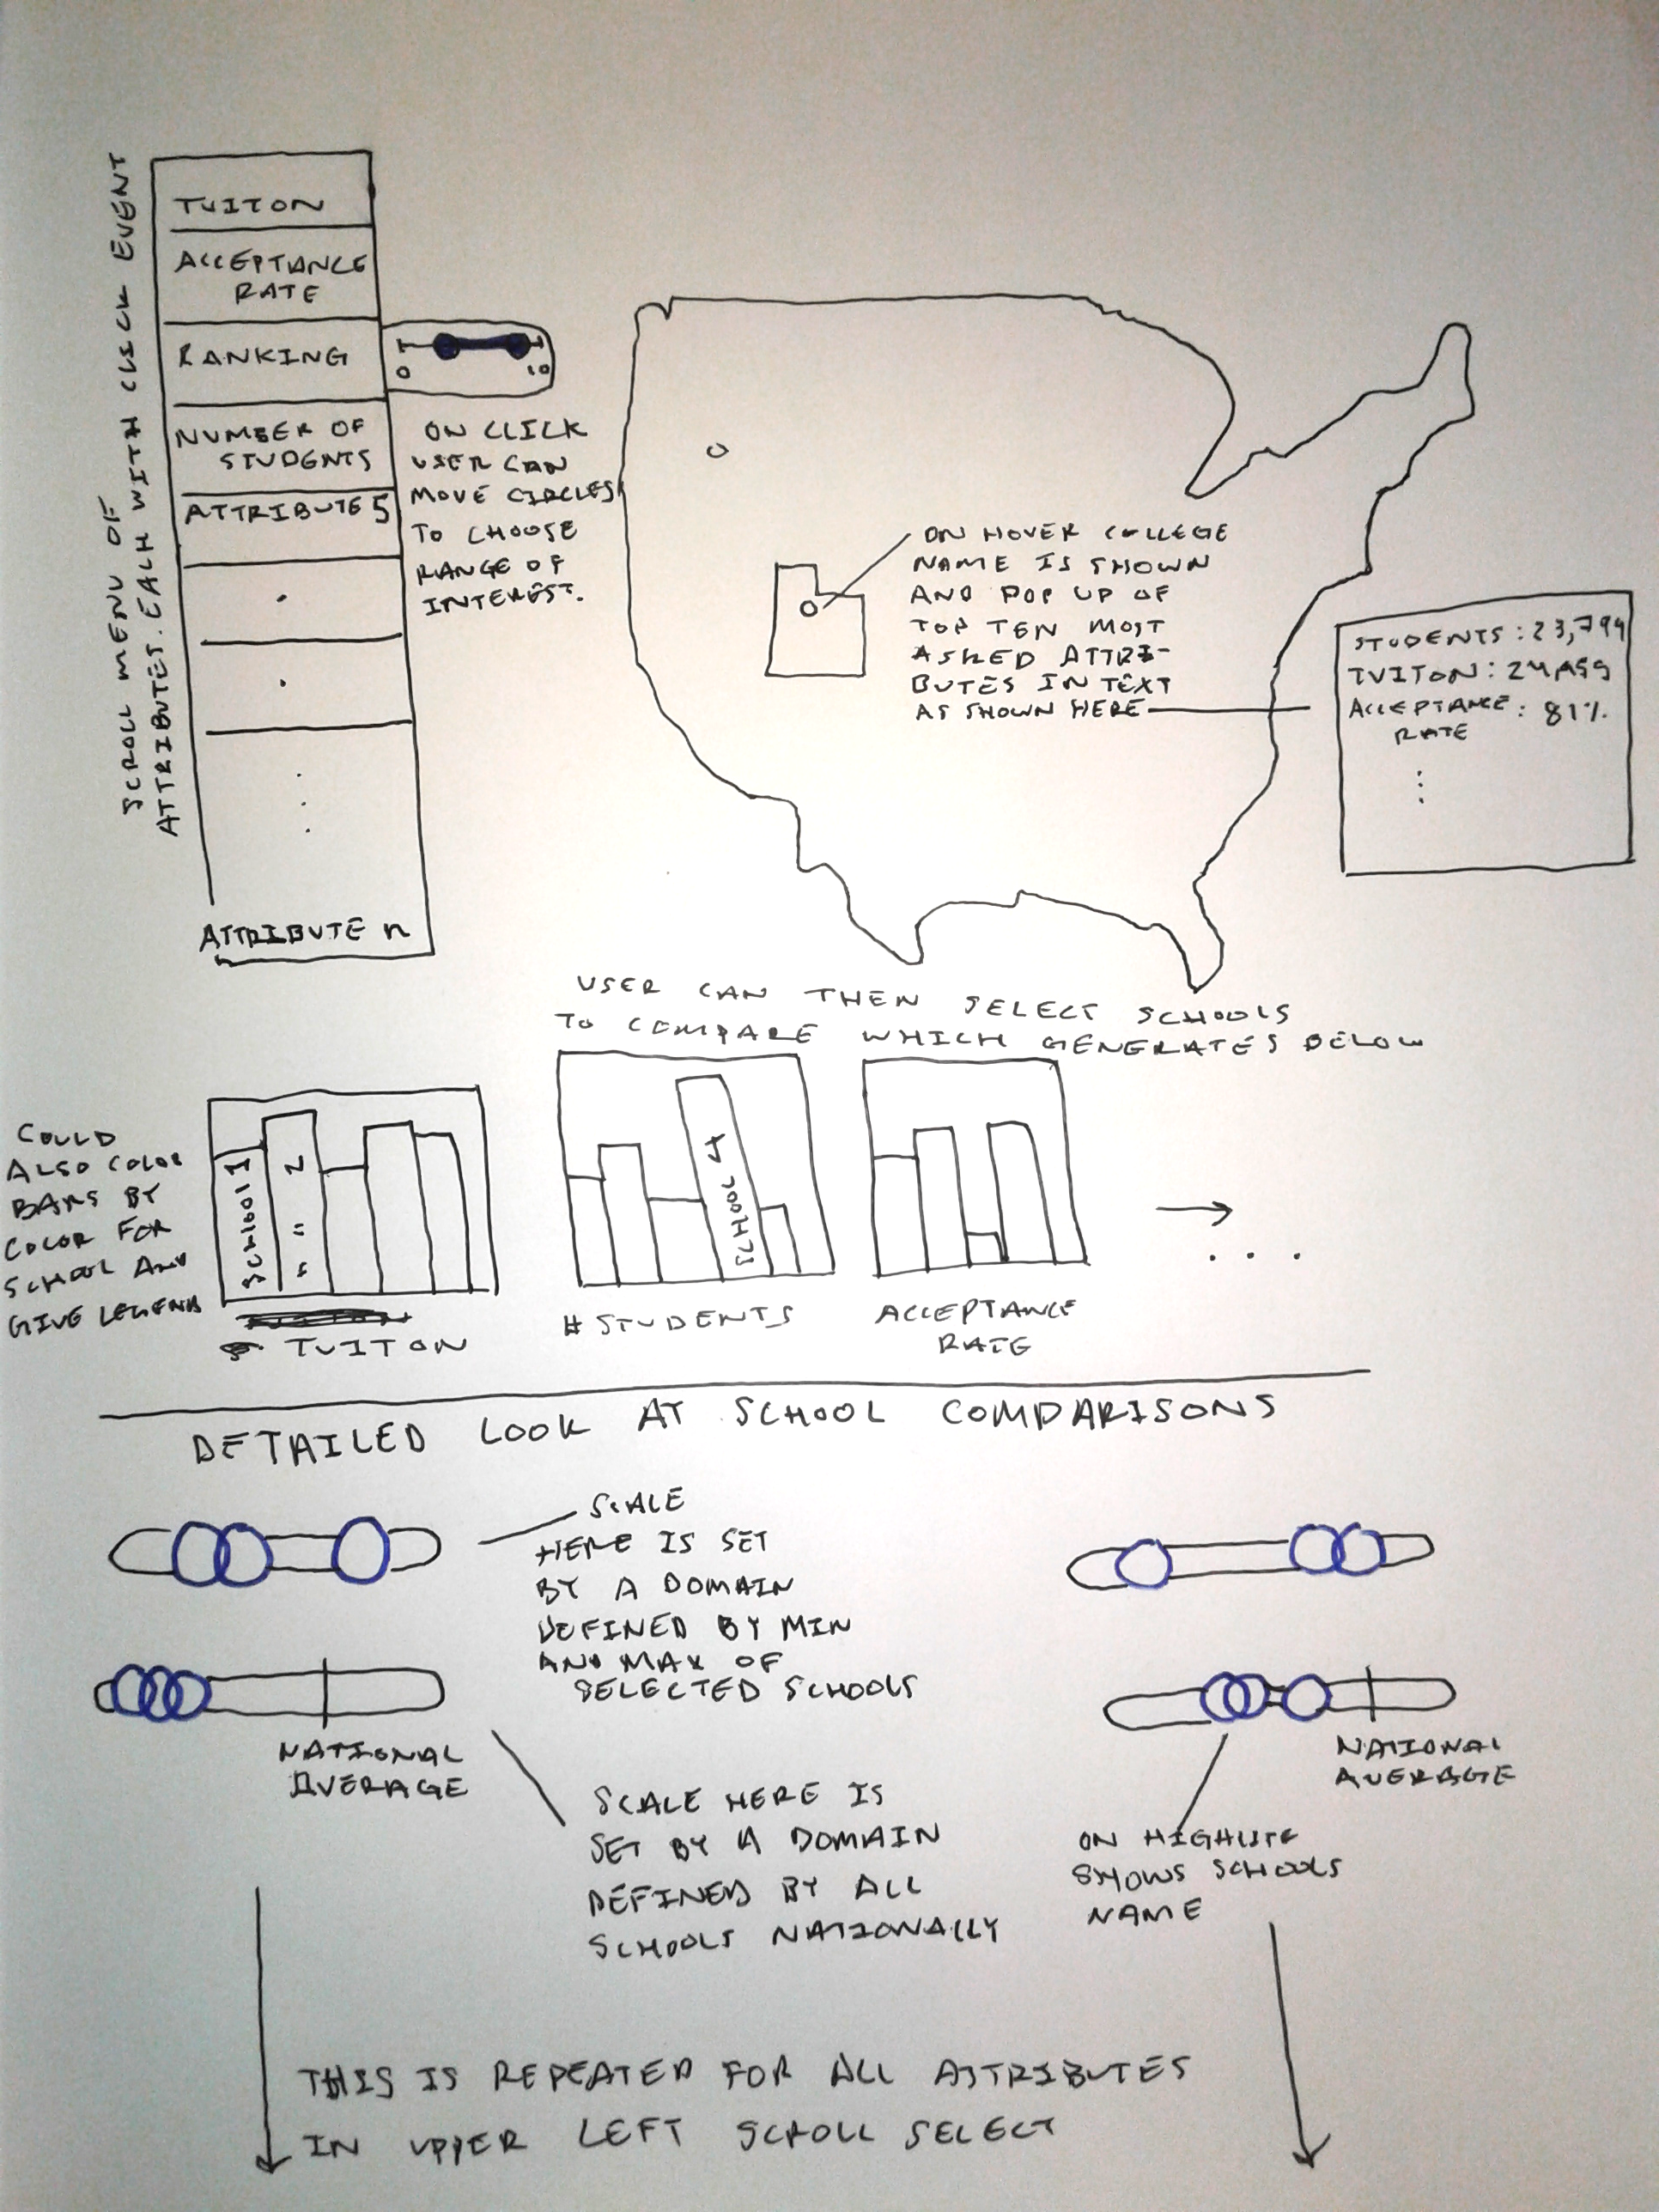
\includegraphics[width=.8\linewidth]{redesignedprojectvisualization.png}
}
\label{Redesigned Project Visualization}
\end{figure}

\end{document}




%%% Local Variables:
%%% mode: latex
%%% TeX-master: t
%%% End:
